\documentclass[a4paper, 12pt]{article}
%\usepackage[T1]{fontenc}
\usepackage[left=2cm,right=2cm,top=2cm,bottom=2cm,includeheadfoot]{geometry}
\usepackage[utf8]{inputenc}
\usepackage[ngerman]{babel}
\usepackage{enumitem}
\usepackage{pdfpages}
\usepackage{ulem} 
\usepackage{graphicx}
\usepackage{caption}
\usepackage{subcaption}
\usepackage{listings}
\usepackage{verbatim}
\usepackage{fancyhdr}
\usepackage{hyperref}
\lstset{
	language=c++,
	extendedchars=\true,
	inputencoding=utf8,
	basicstyle=\ttfamily\footnotesize,
	identifierstyle=,
	stringstyle=\ttfamily\small, 
	showstringspaces=false,
	commentstyle=\color{codegreen},
	keywordstyle=\color{blue},
	stringstyle=\color{codegray}, 
	breakatwhitespace=false,         
	breaklines=true, 
	captionpos=b,                    
	keepspaces=true,                 
	numbers=left,                    
	numbersep=5pt,                  
	showspaces=false,                
	showstringspaces=false,
	showtabs=false,                  
	tabsize=2,
	aboveskip=1em,
}
\usepackage{color}
\usepackage{comment}


\definecolor{codegreen}{rgb}{0,0.6,0}
\definecolor{codegray}{rgb}{0.5,0.5,0.5}
%\definecolor{backcolour}{rgb}{0.95,0.95,0.92}

\pagestyle{fancy}
\lhead[Sascha Beyer, David Schneebauer]{Sascha Beyer, David Schneebauer}
\chead[Projektarbeit Hurace]{Projektarbeit Hurace}
\rhead[SWK5 GRP1 SEBakk BB WS18-19]{SWK5 GRP1 SEBakk BB WS18-19}

%opening
\title{Projektarbeit Hurace}
\author{Sascha Beyer, David Schneebauer}
\date{\today{}, Hagenberg}

\begin{document}
	\maketitle
	\tableofcontents
	\newpage
	\section{Ausbaustufe 1}
	\subsubsection{Datenbankmodell}

	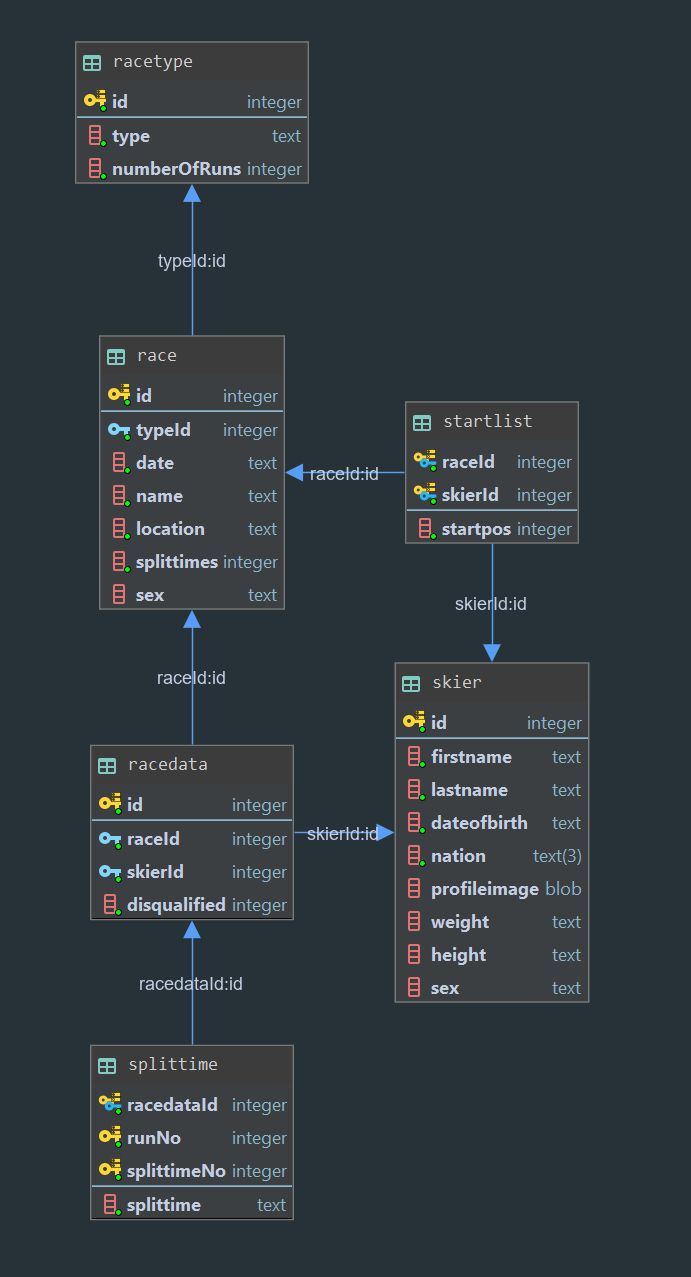
\includegraphics[width=.7\textwidth]{img/huraceDB.png}
	%\lstinputlisting[language=Java]{../Dal/Interface/IRaceDao.cs}
	%\newpage
	%\lstinputlisting[language=Java]{../src/queues/DHeapQueue.java}
	%\newpage
	\newpage
	\subsubsection{Datenbankzugriffsschicht}
	Zur persistierung der Daten wird eine SQLite Datenbank verwendet. Zur Herstellung der Verbindung wird das Factory Pattern verwendet. Über eine Konfigurationsdatei werden Informationen zum Datenbanktyp zur Verfügung gestellt. Für jede Entität sind Dao Klassen implementiert. Diese stellen Methoden für Operationen auf der Datenbank zur Verfügung. Um generisch zu bleiben wird gegen Interfaces implementiert.
	\newline
	 
	%\includegraphics[width=.8\textwidth]{img/main_1.png}
	%\\
	%\includegraphics[width=.8\textwidth]{img/main_2.png}
	%\\
	%\includegraphics[width=.8\textwidth]{img/main_3.png}
	\textbf{IRaceDao}
	\lstinputlisting[language=c++]{../Core.Dal/Interface/IRaceDao.cs}
	\textbf{IRaceDataDao}
	\lstinputlisting[language=c++]{../Core.Dal/Interface/IRaceDataDao.cs}
	\textbf{IRaceTypeDao}
	\lstinputlisting[language=c++]{../Core.Dal/Interface/IRaceTypeDao.cs}
	\textbf{ISkierDao}
	\lstinputlisting[language=c++]{../Core.Dal/Interface/ISkierDao.cs}
	\textbf{ISplittimeDao}
	\lstinputlisting[language=c++]{../Core.Dal/Interface/ISplittimeDao.cs}
	\textbf{IStartListDao}
	\lstinputlisting[language=c++]{../Core.Dal/Interface/IStartListDao.cs}
	
	Um mit schlüssigen Daten arbeiten zu können wurden Importer geschrieben die diese Generieren und in der Datenbank speichern.
	
	\subsection{UnitTests}
	Die entsprechenden Dao Klassen und wurden zusammen mit der restlichen Datenbankzugriffsschicht getestet. 
	\newline
	\newline
	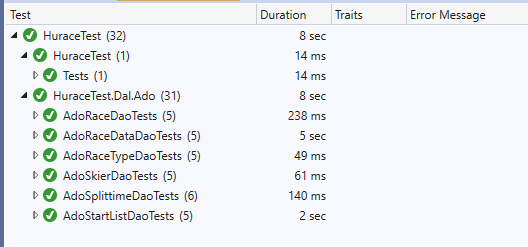
\includegraphics[width=.7\textwidth]{img/UnitTests.png}
	
	\section{Ausbaustufe 2}
	\subsubsection{User Interface}
	
	Damit die optische Komponente einen guten Anstrich bekommt haben wir uns entschieden Material Design zu verwenden, dieses wurde als Nuget Package hinzugefügt und eingebunden, hierbei haben wir uns für das DarkTheme entschieden. Das UI ist nach dem MVVM Muster gebaut und verwendet dessen Vorteile.\\
	Da der Code sehr umfangreich ist wurde dieser nicht in dieses Dokument eingepflegt.\\
	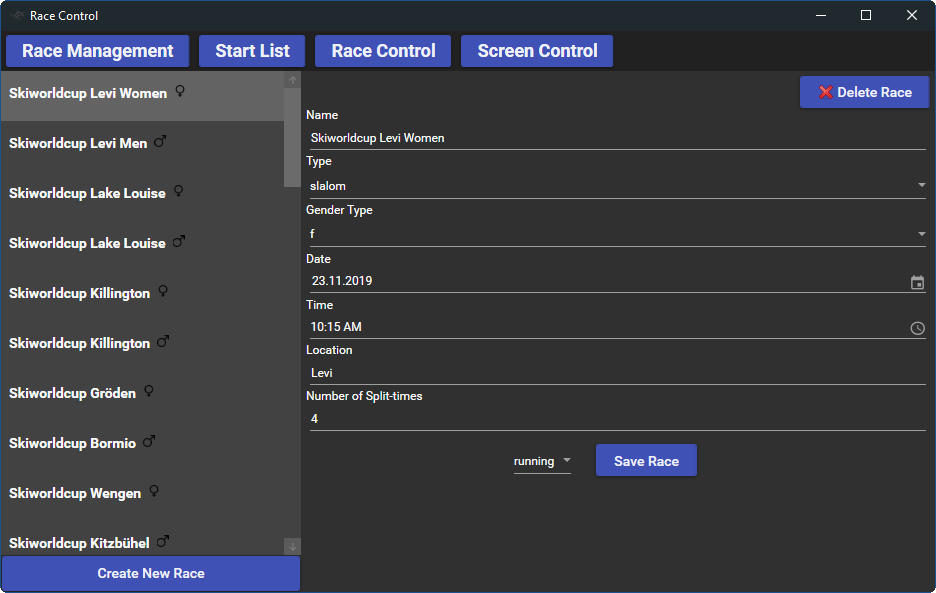
\includegraphics[width=.7\textwidth]{img/ui1.png}\\
	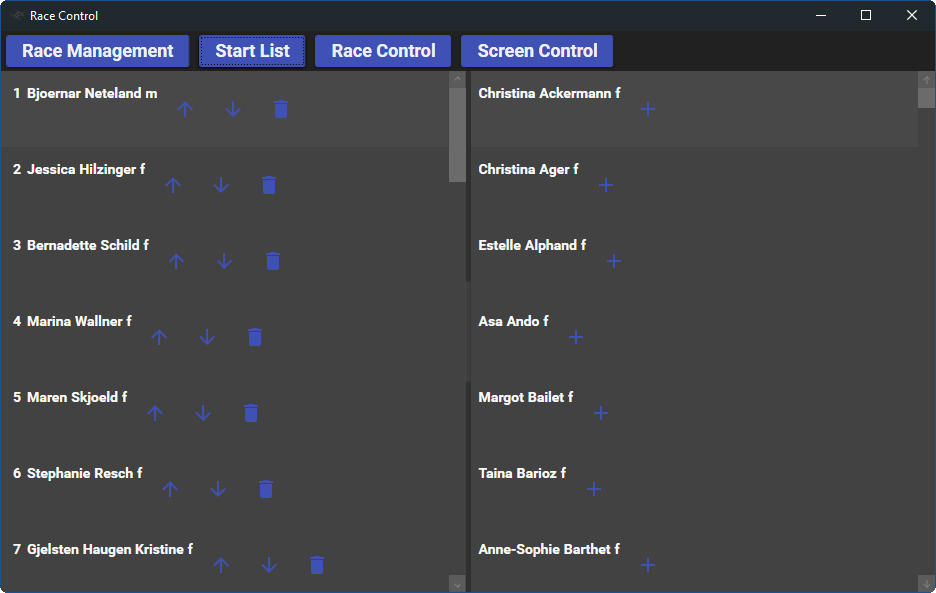
\includegraphics[width=.7\textwidth]{img/ui2.png}\\
	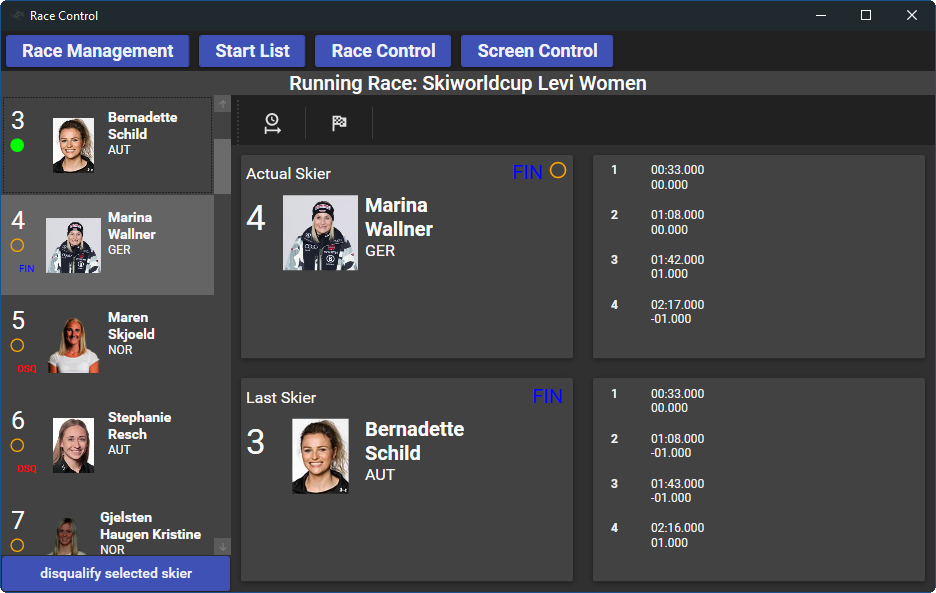
\includegraphics[width=.7\textwidth]{img/ui3.png}\\
	
	
	\newpage
	\subsubsection{Core Logic}
	Um eine Abtrennung der Logik von der Datenbankschicht zu schaffen wurden Interfaces verwendet damit die Datenbankschicht einfach ausgetauscht werden kann. Um die Daten sauber dem UI bereitzustellen wurden Models verwendet um das MVVM Muster umzusetzen.
	\newline
	
	\textbf{IRaceControlLogic}
	\lstinputlisting[language=c++]{../Core.Logic/Interface/IRaceControlLogic.cs}
	\textbf{IRaceManagementLogic}
	\lstinputlisting[language=c++]{../Core.Logic/Interface/IRaceManagementLogic.cs}
	\textbf{IScreenControl}
	\lstinputlisting[language=c++]{../Core.Logic/Interface/IScreenControl.cs}
	\textbf{IStartListLogic}
	\lstinputlisting[language=c++]{../Core.Logic/Interface/IStartListLogic.cs}
	
	
	\subsection{UnitTests}
	Zum Testen der Logik wurde das Mocking Framework Moq verwendet, dieses bietet die Möglichkeit die Datenbankschickt mit gemockten Daten zu abstrahieren wenn man diese mittels Interfaces implementiert hat.
	
	Beispieltests:
	\textbf{IStartListLogic}
	\lstinputlisting[language=c++]{../HuraceTest/RaceManagementLogicTests.cs}
	
	
	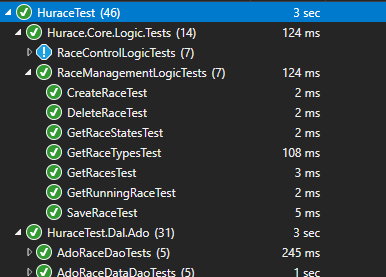
\includegraphics[width=.7\textwidth]{img/UnitTests2.png}

	\newpage	
\end{document}